%-----------------------------------------------------------------------------
%               Template for LaTeX Class/Style File
% Name:         sigplanconf-template.tex
% Purpose:      A template for sigplanconf.cls, which is a LaTeX 2e class
%               file for SIGPLAN conference proceedings.
% Author:       Paul C. Anagnostopoulos
%               Windfall Software
%               978 371-2316
%               paul@windfall.com
% Created:      15 February 2005
%-----------------------------------------------------------------------------

\documentclass[preprint]{sigplanconf}%
\usepackage{amsmath}
\usepackage{amsfonts}
\usepackage{amssymb}
\usepackage{amsthm}
\usepackage{graphicx}
\usepackage{fancyvrb}
\usepackage[dvipsnames]{xcolor}
\usepackage{url}
\usepackage[numbers]{natbib}
\usepackage{subfig}%
\setcounter{MaxMatrixCols}{30}
%TCIDATA{OutputFilter=latex2.dll}
%TCIDATA{Version=5.50.0.2953}
%TCIDATA{LastRevised=Monday, September 22, 2008 11:56:11}
%TCIDATA{<META NAME="GraphicsSave" CONTENT="32">}
%TCIDATA{<META NAME="SaveForMode" CONTENT="1">}
%TCIDATA{BibliographyScheme=Manual}
%BeginMSIPreambleData
\providecommand{\U}[1]{\protect\rule{.1in}{.1in}}
%EndMSIPreambleData
\theoremstyle{remark}
\newtheorem{theorem}{Theorem}
\newtheorem{example}{Example}
\newtheorem{lemma}[theorem]{Lemma}
\renewcommand{\theFancyVerbLine}{\textcolor{gray}{\scriptsize\arabic{FancyVerbLine}}}
\newcommand{\printProgram}[1]{\VerbatimInput[numbers=left,numbersep=5pt,xleftmargin=20pt,
formatcom=\color{Brown},fontsize=\small,
frame=leftline,rulecolor=\color{gray}
]{#1}
}
\newcommand{\printOutput}[1]{\VerbatimInput[formatcom=\color{Brown},fontsize=\small,xleftmargin=20pt,
frame=leftline,rulecolor=\color{gray}
]{#1}
}
\newcommand{\printInline}[1]{\Verb+{\color{Brown}#1}+}
\setlength{\jot}{3.0\jot}
\begin{document}
%
%TCIMACRO{\TeXButton{title}{\conferenceinfo{PLDI '09}%
%{June 15--20, 2009, Dublin, Ireland.}
%\copyrightyear{2009}
%\copyrightdata{[to be supplied]}
%\titlebanner{DRAFT---Do not distribute}
%\preprintfooter{Preprint for PLDI '09}
%\title{Automating Mathematical Program Transformations}
%\authorinfo{Author names omitted for review}
%{ABC University}
%{xy@abc.edu}
%\maketitle}}%
%BeginExpansion
\conferenceinfo{PLDI '09}{June 15--20, 2009, Dublin, Ireland.}
\copyrightyear{2009}
\copyrightdata{[to be supplied]}
\titlebanner{DRAFT---Do not distribute}
\preprintfooter{Preprint for PLDI '09}
\title{Automating Mathematical Program Transformations}
\authorinfo{Author names omitted for review}
{ABC University}
{xy@abc.edu}
\maketitle
%EndExpansion
%

%TCIMACRO{\TeXButton{begin abstract}{\begin{abstract}}}%
%BeginExpansion
\begin{abstract}%
%EndExpansion


Mathematical programs (MPs) are a class of constrained optimization problems.
Various sub-classes are defined by specifying the constraint forms allowed.
For example, linear programs allow only linear equations and inequalities over
the reals, mixed-integer programs also allow integers, and disjunctive
programs allow disjunctive constraints. Algorithms for solving MPs rely
heavily on various transformations between these and other forms. However,
transformations are not automated because MP theory does not presently treat
programs as syntactic objects. Current definitions are given on canonical
matrix forms that enable rigorous numerical analysis, but do not support
automation nor even manual transformation of the natural syntax that programs
are actually written in. We begin by briefly reviewing an MP\ language
previously developed by us, which includes several intuitive constraint forms
that are however not accepted by state-of-the-art algorithms. Our main focus
is on defining a transformation to pure mixed-integer programs, for which
there are solvers. The principle result is the syntactic formalization of the
convex-hull method, big-M method, etc.%

%TCIMACRO{\TeXButton{end abstract}{\end{abstract}}}%
%BeginExpansion
\end{abstract}%
%EndExpansion
%

%TCIMACRO{\TeXButton{keywords}{\category{D}{3}{}
%\terms disjunctive constraint, convex-hull
%\keywords convex-hull transformation, mathematical program}}%
%BeginExpansion
\category{D}{3}{}
\terms disjunctive constraint, convex-hull
\keywords convex-hull transformation, mathematical program%
%EndExpansion


\section{Introduction}

NEED TO SHORTEN INTRO.

The equations governing engineering systems rarely dictate a unique solution.
Usually, a designer needs to find the optimal solution amongst a space of
feasible ones. For example, a chemical plant might be required to produce
product at a certain rate. In addition it must not violate safety
requirements---e.g. the temperature of reactors must not get too high, and of
course, physical laws must be obeyed---e.g. total mass entering a reactor must
equal that exiting. Despite these constraints, there are an infinite number of
ways to design and operate such a plant. Each choice incurs different capital
and operating costs. The question then is how to find the solution that
minimizes cost amongst those satisfying the hard constraints.

Such constrained optimization problems are often expressed as mathematical
programs (MPs), which consist of a numerical objective that is to be maximized
(or minimized) subject to some constraints. The nature of the constraints
allowed is a key issue affecting both the kinds of systems that can be
represented and the efficiency of algorithms. An MP is more specifically
called a linear program (LP) when the constraints are linear algebraic
equations and inequalities on the reals. A mixed-integer linear program (MILP)
additionally allows restricting variables to be integer valued. This allows a
broader class of systems to be represented. Other variations allow
disjunctions over equations, and also Boolean expressions.

The standard definition of a linear program is%
\begin{equation}
\mathrm{max}\left\{  cx:Ax\leq b,x\in\mathbb{R}^{n}\right\}
\label{LP matrix def}%
\end{equation}
where $c$ is a $1\times n$ dimensional coefficient vector, $x$ is an
$n\times1$ vector of real valued variables, $A$ is an $m\times n$ coefficient
matrix, and $b$ is an $m\times1$ vector of constants. Thus, $cx$ is a scalar,
and the matrix inequality $Ax\leq b$ represents $m$ individual inequalities.
The inequalities represent a polyhedron, such as region $R^{1}$ or $R^{2}$ in
Figure \ref{ex_DP}, and is called the feasible space of the LP. The objective
$cx$ has a value for each point in the polyhedron, and the solution to an
LP\ provides that point in the polyhedron for which $cx$ is maximum. There
might not be a maximum if the polyhedron is open.%
%TCIMACRO{\TeXButton{figure: ex_DP_imgs}{\begin{figure*}[bth]
%\subfloat[Feasible region.]{\label{ex_DP}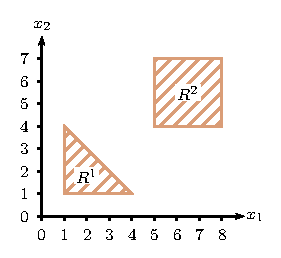
\includegraphics{img/ex_DP.eps}%
%}\hfill\subfloat[Big-M relaxation.]{\label{ex_bigM_DP}\includegraphics
%{img/ex_bigM_DP.eps}}\hfill\subfloat[Convex hull relaxation.]{\label
%{ex_cvx_DP}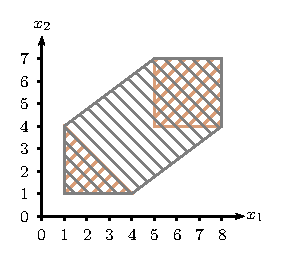
\includegraphics{img/ex_cvx_DP.eps}}
%\caption{A disjunctive region and two reformulations.}
%\label{ex_DP_imgs}
%\end{figure*}}}%
%BeginExpansion
\begin{figure*}[bth]
\subfloat[Feasible region.]{\label{ex_DP}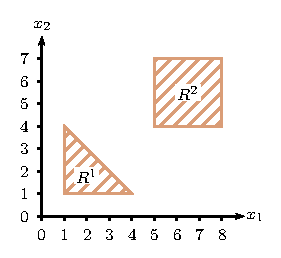
\includegraphics{img/ex_DP.eps}%
}\hfill\subfloat[Big-M relaxation.]{\label{ex_bigM_DP}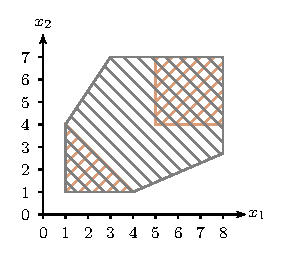
\includegraphics
{img/ex_bigM_DP.eps}}\hfill\subfloat[Convex hull relaxation.]{\label
{ex_cvx_DP}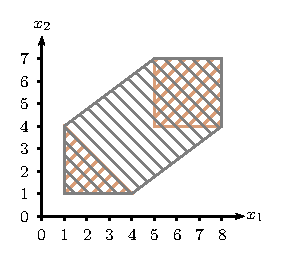
\includegraphics{img/ex_cvx_DP.eps}}
\caption{A disjunctive region and two reformulations.}
\label{ex_DP_imgs}
\end{figure*}%
%EndExpansion


Representing discrete choices, purchasing reactor A or reactor B, requires a
more expressive language than LP. Discrete decisions affect real valued
variables. Reactor A may be able to withstand higher temperatures than reactor
B, and might cost more. What is needed is a way to associate polyhedra with
the different discrete choices. The feasible space is then a union of
polyhedra, such as $R^{1}\cup R^{2}$ in Figure \ref{ex_DP}. There are two
rather distinct methods for accomplishing this. One enriches the types and the
other the constraint forms.

A mixed-integer linear program (MILP) allows variables to be integer or real
valued. The standard definition \cite{Nemhauser1999}\ of an MILP is%
\begin{equation}
\mathrm{max}\left\{  cx+hy:Ax+Gy\leq b,x\in\mathbb{R}^{n},y\in\mathbb{Z}%
^{p}\right\}  \label{MILP matrix def}%
\end{equation}
where $x$ and $y$ represent vectors of real and integer variables,
respectively. Let $x_{1}$ represent temperature, and let $y_{1}=1$ mean
reactor A is purchased and $y_{2}=1$ mean reactor B is purchased. Then, the
inequalities%
\begin{subequations}
\begin{align}
0  &  \leq y_{1}\leq1\\
0  &  \leq y_{2}\leq1\\
y_{1}+y_{2}  &  =1\\
x_{1}  &  \leq1000y_{1}+800y_{2}%
\end{align}
correctly model the reactor example. Firstly, the integer variables $y_{i}$
are required to take only the value $0$ or $1$. The third constraint requires
their sum to be $1$, meaning exactly one of $y_{1},y_{2}$ can be $1$ and the
other must be $0$. The last constraint reduces to $x_{1}\leq1000$ if reactor A
is purchased or $x_{1}\leq800$ if reactor B is purchased, exactly as desired.

Experienced mathematical programmers could have quickly formulated the model
for this toy problem, but we can see that some amount of ingenuity is
required. Integers are not an intuitive model of discrete choice, and become
prohibitively difficult for larger problems. Enriching LP\ with disjunctive
constraints leads to more compact and comprehensible models
\cite{Balas1974,r3000}. The constraint%
\end{subequations}
\begin{equation}
\left(  x_{1}\leq1000\right)  \vee\left(  x_{1}\leq800\right)
\label{reactor_disj}%
\end{equation}
more elegantly communicates the same result as the previous MILP\ constraints.
Another extension known as generalized disjunctive programs also allows
Boolean expressions and discrete variables within disjuncts \cite{r3000}.
(Boolean expressions are statements on Boolean variables, as opposed to the
conjunctive-disjunctive constraints we have been discussing, which are
statements on reals.)

There are however few algorithms for solving disjunctive programs and its
variations, while there is a large body of literature for solving MILPs. The
usual strategy thus is to convert disjunctive programs to equivalent
mixed-integer forms, which is possible due to Balas's convex-hull method, the
big-M method, and other techniques \cite{Balas1974,Balas1998,r3000}.

Roughly, the idea is to associate an integer binary variable $y_{i}\in\{0,1\}$
with each $i^{\text{th}}$disjunct of a disjunction, and to replace the
disjunction with conjunction. Just one $y_{i}$ is required to be $1$ and only
the constraints of the corresponding disjunct are enforced. Disjuncts
$j\not =i$ get reduced to trivial tautologies. A naive method is to multiply
the inequalities in each disjunct by its corresponding binary variable.
Disjunction (\ref{reactor_disj}) becomes the conjunction%
\begin{subequations}
\begin{align}
x_{1}y_{1}  &  \leq1000y_{1}\\
x_{1}y_{2}  &  \leq800y_{2}\\
y_{1}+y_{2}  &  =1\\
0  &  \leq y_{1}\leq1\\
0  &  \leq y_{2}\leq1
\end{align}
Now if $y_{1}=0$ and $y_{2}=1$, these reduce to $0\leq0$ and $x_{1}\leq800$.
As desired, only the second disjunct is being enforced, while the first is
eliminated. Conversely, if $y_{1}=1$ and $y_{2}=0$.

Unfortunately, this simple transformation is also a very poor one. Multiplying
two variables creates nonlinear and possibly nonconvex programs, which are
significantly more complex to solve. The big-M method is more complex but with
the benefit of producing linear mixed-integer constraints. In most cases, the
convex-hull method is even better. It produces linear constraints too, but is
also a tighter formulation than big-M. During execution, MILP algorithms allow
integer variables to take any real value, called relaxation. Tightness refers
to the size of the resulting feasible space and significantly effects
computation times. Figures \ref{ex_bigM_DP} and \ref{ex_cvx_DP} show this
space for the big-M and convex-hull methods, respectively. We can see the
latter is smaller. Indeed it is the smallest convex region covering the
original disjoint regions, and hence the name of the transformation producing it.

Unfortunately, the convex-hull method is difficult to apply on even small
problems. Despite its well known utility and wide impact on the solution of
mixed-integer programs, its use has been limited to experts familiar with
Balas's theory. Even they are restricted since several pages of algebra can be
required to transform disjunctions with a moderate number of sub-terms.

The canonical matrix form of a disjunctive constraint is%
\end{subequations}
\begin{equation}
\left[  A^{1}x\leq b^{1}\right]  \vee\left[  A^{2}x\leq b^{2}\right]  ,
\label{Binary DP}%
\end{equation}
where $A^{i}$ is an $m^{i}\times n$ coefficient matrix, $x$ is an $n\times1$
vector of real variables, and $b^{i}$ is an $m^{i}\times1$ vector of
constants. The convex hull method states that (\ref{Binary DP}) can be
transformed into the equivalent mixed-integer constraints
\begin{subequations}
\label{Binary cvx DP}%
\begin{align}
A^{1}\bar{x}^{1}  &  \leq b^{1}\lambda_{1}\\
A^{2}\bar{x}^{2}  &  \leq b^{2}\lambda_{2}\\
\lambda_{1}+\lambda_{2}  &  =1\\
x  &  =\bar{x}^{1}+\bar{x}^{2}%
\end{align}
where $\lambda_{i}\in\left\{  0,1\right\}  $. In each of the $i^{\text{th}}$
disjuncts, vector $x$ has been replaced with a new vector of variables
$\bar{x}^{i}$. This causes the inequalities of each disjunct to be
disaggregated, meaning they have no variables in common. For this reason, the
$\bar{x}^{i}$'s are called the disaggregated variables. Finally, the original
$x$ is defined to be a sum of the new $\bar{x}^{i}$'s. The validity of the
transformation and proof that it does represent the convex-hull is discussed
by Balas \cite{Balas1974,Balas1998}.

On matrix forms, the method is speciously simple, but further consideration
reveals the complexity of which there are two sources: some details are
omitted in the given transformation and MP\ models are in fact never written
in matrix form\footnote{Constraint declarations are made manageable by the use
of index sets, which we are not considering in the current work. Their
inclusion would further motivate our call for a syntactic mechanization of
MP\ transformations.}. In practice, the $m^{i}$ inequalities of each disjunct
would be written out separately, and in general more than two disjuncts are of
course allowed. Thus, in practice $%
%TCIMACRO{\tsum _{i}}%
%BeginExpansion
{\textstyle\sum_{i}}
%EndExpansion
m^{i}$ individual constraints must be manipulated. The $x$'s would in fact
have $n$ unique names, and $2n+2$ new variable names have to be generated.
Firstly, (\ref{Binary cvx DP}) fails to mention how these variables are
introduced. Remarkably, both the theoretical definitions of MP and the tools
supporting them do not support locally scoped variable declarations, due to
the lack of a syntactic perspective in this field. These variable names must
thus be unique across the entire program.

There is also a precondition that (\ref{Binary DP}) must satisfy before
applying the convex-hull method. The region represented by each disjunct must
be bounded. Balas assumes that a separate bounded inequality $A^{\prime}x\leq
b^{\prime}$ is also part of the model. Disjunction (\ref{Binary DP}) is first
converted to%
\end{subequations}
\begin{equation}
\left[
\begin{array}
[c]{c}%
A^{\prime}x\leq b^{\prime}\\
A^{1}x\leq b^{1}%
\end{array}
\right]  \vee\left[
\begin{array}
[c]{c}%
A^{\prime}x\leq b^{\prime}\\
A^{2}x\leq b^{2}%
\end{array}
\right]  ,
\end{equation}
further increasing the number of constraints being manipulated to $%
%TCIMACRO{\tsum _{i}}%
%BeginExpansion
{\textstyle\sum_{i}}
%EndExpansion
(m^{\prime}+m^{i})$. Often $m^{\prime}$ equals $2n$ because a lower and upper
bound is provided for each variable separately. Presently, maintenance of
variable bounds has been treated informally, but we provide a precise
mechanism for doing so, allowing the automatic generation of the required inequalities.

Finally, even as a canonical form, (\ref{Binary DP}) is not complete. It
assumes a disjunctive normal form, but nested disjunctions are common in
practice. Converting to disjunctive normal form greatly increases the number
of constraints. Alternatively, the transformation can be first applied to the
inner-most disjunction, working outward, but this also compounds the number of
constraints at each application. A disjunction with just three levels of
nesting and only a few constraints in each disjunct can require a few pages of
algebra \cite{h3000}. Automation is clearly called for.

There are several widely used languages that support a more natural input
syntax \cite{Kallrath2004}, the dominant ones being GAMS \cite{Bisschop1982},
AMPL \cite{Fourer1990}, Mosel \cite{Colombani2002}, and OPL
\cite{vanHentenryck1999}. However, none have much support for automated
program transformations. Partly this is because the languages themselves are
not designed with formal methods. Their view is that a computer language is a
mere notational interface for the \textquotedblleft true\textquotedblright%
\ matrix based definitions of an MP. Indeed, the earliest efforts referred to
this topic as matrix generation; the purpose was to immediately parse input
into the matrices of definitions (\ref{LP matrix def}) and
(\ref{MILP matrix def}).

Matrices cannot however represent disjunctive or Boolean expressions, so the
issue of transforming them cannot even be addressed. Recent attempts to extend
the syntax have had little success due to the lack of a supporting theory. For
example, it is not difficult to find examples of disjunctive constraints being
transformed erroneously (see Anonymous's dissertation \cite{a3000} for
examples). Furthermore, no single language supports the full range of desired
constraint forms: mixed-integer, disjunctive, Boolean, and arbitrary mixtures
of them.

In the next section we briefly review the MP language defined in Anonymous's
thesis \cite{a3000}. Unlike previous languages, its type system and semantics
have been formally defined. Enabled by this, the present work provides a
formalization of MP transformations currently performed manually. The source
language contains the rich variety of constraints used by MP practitioners,
but that are not supported in previous languages nor accepted by solvers. The
target language is MILP, for which good algorithms do exist. The main
transformation required is that of disjunctive constraints, for which we have
chosen the convex-hull method. The relatively simpler transformation of
Boolean expressions is also provided.

\section{Mathematical Programming Language}

DEFINITIONS OF THIS SECTION SHOULD BE IN A FIGURE. MINIMIZE DISCUSSION OF TYPE
SYSTEM AND REAL COMPUTATION.

Our mathematical programming language consists of types $\tau$, expressions
$e$, constraints (called propositions in logic) $c$, and programs $p$. The
syntax is%
\begin{equation}
\tau::=\mathtt{real}\mid\mathtt{bool}%
\end{equation}%
\begin{align}
e  &  ::=x\mid r\mid\mathtt{true}\mid\mathtt{false}\nonumber\\
&  \mid-e\mid e_{1}+e_{2}\mid e_{1}-e_{2}\mid e_{1}\ast e_{2}\nonumber\\
&  \mid\mathtt{not}\,e\mid e_{1}\,\mathtt{or}\,e_{2}\mid e_{1}\,\mathtt{and}%
\,e_{2}%
\end{align}%
\begin{align}
c  &  ::=\mathtt{T}\mid\mathtt{F}\nonumber\\
&  \mid\mathtt{isTrue}\;e\mid e_{1}=e_{2}\mid e_{1}\leq e_{2}\nonumber\\
&  \mid c_{1}\vee c_{2}\mid c_{1}\wedge c_{2}\nonumber\\
&  \mid\exists x\!:\!\tau\centerdot c
\end{align}%
\begin{equation}
p::=\mathrm{max}_{x_{1}:\tau_{1},\ldots,x_{m}:\tau_{m}}\left\{  e\mid
c\right\}
\end{equation}


The types are $\mathtt{real}$ and $\mathtt{bool}$; integers will be discussed
shortly. Expressions include variables, rational constants $r$, Boolean
constants, and the usual numeric and Boolean operators. We wish only to
support linear terms, and so the restriction on $e_{1}\ast e_{2}$ is that
$e_{1}$ has no free variables. Nonlinear programs are certainly important, but
the convex-hull method we are focusing on applies only to linear constraints.

Constraints include propositional constants $\mathtt{T}$ and $\mathtt{F}$,
which are distinct from the Boolean constants $\mathtt{true}$ and
$\mathtt{false}$. The constraint $\mathtt{isTrue}\;e$ lifts Boolean
expressions to the constraint level. Equality and inequality are supported for
real expressions. We can treat $e_{2}\geq e_{1}$ as a synonym for $e_{1}\leq
e_{2}$, but note that MPs do not allow strict inequalities. Correspondingly,
there is no negation at the constraint level. Next, the disjunction $\vee$ and
conjunction $\wedge$ of constraints is provided. Again, these are distinct
from the Boolean operators $\mathtt{or}$ and $\mathtt{and}$. The convex-hull
method applies only to disjunctive constraints and has nothing to do with
Boolean disjunction. Our syntactic separation of these concepts allows our
program transformations to be applied to the correct category of objects.
Finally, variables are introduced through existential quantification.
Universal quantifiers would extend our language to include semi-infinite
programs, an interesting but less developed class of problems.

Programs $p$ are of a single syntactic form $\mathrm{max}_{x_{1}:\tau
_{1},\ldots,x_{m}:\tau_{m}}\left\{  e\mid c\right\}  $ and the definition is
not inductive. This is roughly similar to definition (\ref{MILP matrix def})
but the objective $e$ and constraint $c$ is not in a matrix form. Variables
introduced at the program level behave semantically as those introduced by
existential quantifiers over constraints. The only difference is that they can
also be used in the objective. We can treat $\mathrm{min}_{x_{1}:\tau
_{1},\ldots,x_{m}:\tau_{m}}\left\{  e\mid c\right\}  $ as a synonym for
$\mathrm{max}_{x_{1}:\tau_{1},\ldots,x_{m}:\tau_{m}}\left\{  -e\mid c\right\}
$.

More extensive discussion of the syntax is provided in \cite{a3000}. There,
the type system and semantics are also defined. A cursory overview will
suffice here. Expressions are typed in the usual way. A context%
\begin{equation}
\Gamma::=\bullet\mid\Gamma,x\!:\!\rho
\end{equation}
retains variables' types (variable names are assumed to be unique), and
expressions are assigned a type within a context. Numeric operators require
their sub-expressions to be of type $\mathtt{real}$ and Boolean operators'
sub-expressions must be of type $\mathtt{bool}$. The constraint
$\mathtt{isTrue}\;e$ is well formed only if $e$ is of type $\mathtt{bool}$,
and $e_{1}=e_{2}$ and $e_{1}\leq e_{2}$ are well formed only if $e_{1}$ and
$e_{2}$ are both of type $\mathtt{real}$. The constraint $\exists
x\!:\!\tau\centerdot c$ is well formed if its body $c$ is under the same
context augmented with $x\!:\!\tau$, where $\alpha$-conversion is used as
necessary. A program is well formed if its objective $e$ is of type
$\mathtt{real}$, and its constraint $c$ is well formed, within the context
containing all variables introduced by the program.

Inclusion of the type $\mathtt{real}$ poses complications for the semantics of
this language. We assume a notion of $+$ exists in the meta-language and
simply define the object language's $+$ to coincide with this one. Since we
want our language to represent the existing field of mathematical programming,
we must follow existing practice. Mathematical programming treats numbers
classically. It is assumed that variables can be assigned real values. These
assumptions are not tenable from a computational perspective. An exact
implementation of the semantics of our language, and of existing algorithms
purportedly solving MPs, requires a constructive formulation of the reals, a
significant challenge being addressed by others. Lacking this should not
dissuade automating program transformations; which is a purely syntactic
operation. Real expressions are carried through unaltered.

The convex-hull transformation requires knowledge of variable bounds, and we
have also yet to support integers. We now introduce a slight modification to
the syntax that accomplishes both. Refined types%
\begin{align}
\rho &  ::=\left[  r_{L},r_{U}\right]  \mid\left[  r_{L},\infty\right)
\mid\left(  -\infty,r_{U}\right]  \mid\mathtt{real}\nonumber\\
&  \mid\left\langle r_{L},r_{U}\right\rangle \mid\left\langle r_{L}%
,\infty\right)  \mid\left(  -\infty,r_{U}\right\rangle \mid\mathtt{int}%
\nonumber\\
&  \mid\left\{  \mathtt{true}\right\}  \mid\left\{  \mathtt{false}\right\}
\mid\mathtt{bool}%
\end{align}
can be thought of as subsets of types $\tau$. Square brackets denote real
intervals, and angle brackets integer intervals. Classically, integers are a
subset of the reals.

We now replace type declarations with refined type declarations, which are
present in existential quantifiers and the top program level. Instead of
$\exists x\!:\!\tau\centerdot c$ we allow $\exists x\!:\!\rho\centerdot c$,
and instead of $\mathrm{max}_{x_{1}:\tau_{1},\ldots,x_{m}:\tau_{m}}\left\{
e\mid c\right\}  $ we allow $\mathrm{max}_{x_{1}:\rho_{1},\ldots,x_{m}%
:\rho_{m}}\left\{  e\mid c\right\}  $. This modification does not alter the
type system. It is an annotation in the syntax allowing variable bounds to be
systematically provided. It affects the semantics by restricting the allowed
values of a variable. Thus refined type declarations can be considered an
additional constraint form. Analogously to a context, we define the refined
context%
\begin{equation}
\Upsilon::=\bullet\mid\Upsilon,x\!:\!\rho
\end{equation}
as a list of refined type declarations.

Finally, we define free variables and substitution in the usual way. Let
$FV(e)$ and $FV(c)$ refer respectively to the free variables of an expression
and constraint. For example, $FV(\exists x\!:\!\rho\centerdot
x+(1-y))=\left\{  y\right\}  $ because $x$ is bound within the body of an
existential constraint. Let $\left\{  e/x\right\}  e^{\prime}$ denote the
substitution of $e$ for $x$ in $e^{\prime}$, handling variable capture as
needed. Similarly, $\left\{  e/x\right\}  c$ substitutes $e$ for $x$ in
constraint $c$.

\section{Transforming Syntactic Constructs}

The class of programs covered by $p$ include disjunctive constraints and
Booleans, but most solvers accommodate only mixed-integer linear programming
(MILP) constraints. Formally, we define the MILP\ types $\rho^{\textsc{milp}}$
to be as above but exclude $\left\{  \mathtt{true}\right\}  $, $\left\{
\mathtt{false}\right\}  $, and $\mathtt{bool}$; MILP expressions
$e^{\textsc{milp}}$ disallow Boolean constants and Boolean operators, and
MILP\ constraints $c^{\textsc{milp}}$ disallow $\mathtt{isTrue}\;e$ and
$c_{1}\vee c_{2}$. Essentially, the only constraints included in
$c^{\textsc{milp}}$ are conjunctions of equations and inequalities. Finally,
let $p^{\textsc{milp}}$ refer to programs containing only MILP\ types,
expressions, and constraints.

Our goal now is to provide a method for transforming programs in the source
language $p$ to those in the target language $p^{\textsc{milp}}$, a subset of
the source. We know this can be done, under a mild condition, because of
previous results by \cite{Balas1974}, \cite{r3000}, and others. However, the
transformation procedures in these works have been stated in English. We now
provide a syntactic formalization.

Transforming a program requires transforming the types, expressions, and
constraints that comprise it. We provide a transformation procedure for each
construct in turn.

\subsection{Type Transformation}

Let $\rho\overset{\text{\textsc{rtype}}}{\longmapsto}\rho^{\textsc{milp}}$ be
a binary relation on types meaning the general type $\rho$ can be transformed
to the MILP\ type $\rho^{\textsc{milp}}$. The definition of this judgement is
given by the rules%
\begin{subequations}
\begin{align}
&  \left\{  \mathtt{true}\right\}  \overset{\text{\textsc{rtype}}}%
{\longmapsto}\left\langle 1,1\right\rangle \\
&  \left\{  \mathtt{false}\right\}  \overset{\text{\textsc{rtype}}%
}{\longmapsto}\left\langle 0,0\right\rangle \\
&  \mathtt{bool}\overset{\text{\textsc{rtype}}}{\longmapsto}\left\langle
0,1\right\rangle \\
&  \rho\overset{\text{\textsc{rtype}}}{\longmapsto}\rho\quad\text{other }\rho
\end{align}
Numeric types are allowed in the target language, and thus need not be
transformed. Type $\mathtt{bool}$ is converted into the type $\left\langle
0,1\right\rangle $, which is the set containing the two integers $0$ and $1$.
Type $\left\{  \mathtt{false}\right\}  $ is converted to the singleton set
$\left\langle 0,0\right\rangle $, and $\left\{  \mathtt{true}\right\}  $ into
$\left\langle 1,1\right\rangle $.

Let $\Upsilon\overset{\text{\textsc{ctxt}}}{\longmapsto}\Upsilon
^{\textsc{milp}}$ be a context transformation. Its definition is%
\end{subequations}
\begin{subequations}
\begin{align}
&  \frac{{}}{\bullet\overset{\text{\textsc{ctxt}}}{\longmapsto}\bullet}\\
&  \frac{\Upsilon\overset{\text{\textsc{ctxt}}}{\longmapsto}\Upsilon
^{\textsc{milp}}\quad\rho\overset{\text{\textsc{rtype}}}{\longmapsto}%
\rho^{\textsc{milp}}}{\Upsilon,x\!:\!\rho\overset{\text{\textsc{ctxt}}%
}{\longmapsto}\Upsilon^{\textsc{milp}},x\!:\!\rho^{\textsc{milp}}}%
\end{align}
This simply transforms each of the declared types in a context.

\subsection{Conjunctive Normal Form}

DELETE THIS SECTION. JUST MENTION THAT WE HAVE THIS.

Boolean expressions can be converted into integer constraints, but producing
linear integer constraints requires first converting to conjunctive normal
form (CNF). We discuss this first, and in the next section show how Booleans
can be mapped to integers. The definition of CNF follows the standard idea,
but we do not require the atomic forms that are sometimes defined. Also we
will need to partition CNF forms into two disjoint sets, those involving
conjunction and those not.

Let $e\;$\textsc{literal} mean expression $e$ is a literal. Expressions
satisfying this judgement are $x$, $\mathtt{true}$, $\mathtt{false}$, and
$\mathtt{not}\,e^{\prime}$ when $e^{\prime}\;$\textsc{literal}. Disjunctive
literal forms are defined by the judgement $e\;$\textsc{dlf}, which is
satisfied by all \textsc{literal}\ forms, as well as $e_{1}\,\mathtt{or}%
\,e_{2}$ when $e_{1}\;$\textsc{dlf} and $e_{2}\;$\textsc{dlf}. Finally, the
judgement $e\;$\textsc{cnf} includes all \textsc{dlf} expressions as well as
$e_{1}\,\mathtt{and}\,e_{2}$ when $e_{1}\;$\textsc{cnf} and $e_{2}%
\;$\textsc{cnf}. CNF expressions include DLF\ expressions and conjunctive
expressions $e_{1}\,\mathtt{and}\,e_{2}$. The latter we call
CONJ\ expressions. Precisely, $e\;$\textsc{conj} includes those expressions
satisfying $e\;$\textsc{cnf} but not $e\;$\textsc{dlf}. We will see that
CONJ\ expressions must be transformed differently from DLF expressions if we
are to produce linear constraints.

Let $e_{1}\curvearrowright e_{2}$ be a judgement relating an arbitrary Boolean
expression $e_{1}$ to its conjunctive normal form $e_{2}$. Its definition is
not just inductive on $e_{1}$. The form of $e_{1}$ is first considered, but
further induction on its nested expressions is required. The definition of
$\curvearrowright$ is%
\end{subequations}
\begin{subequations}
\begin{align}
&  \frac{e\;\text{\textsc{cnf}}}{e\curvearrowright e}\\
&  \frac{e_{1}\;\lnot\text{\textsc{cnf}}\quad e_{1}\curvearrowright_{\ast
}e_{2}}{e_{1}\curvearrowright e_{2}}%
\end{align}
If the expression is already in \textsc{cnf}, nothing is done, i.e. the
relation is reflexive. Expressions not in \textsc{cnf} are passed to an
auxiliary relation $e_{1}\curvearrowright_{\ast}e_{2}$, which is defined only
for $e_{1}$ such that $e_{1}\;\lnot$\textsc{cnf}.

The definition of $e_{1}\curvearrowright_{\ast}e_{2}$ is inductive on $e_{1}$
and its nested forms. Only expression forms which could possibly be Boolean
need to be considered---there are six: $x$, $\mathtt{true}$, $\mathtt{false}$,
$\mathtt{not}\,e$, $e_{1}\,\mathtt{or}\,e_{2}$, and $e_{1}\,\mathtt{and}%
\,e_{2}$. Three have no nested expressions, one is a unary operator, and two
are binary operators. Thus, up to $1+1+1+6+36+36=81$ rules could be needed.
The total is reduced because some are already in \textsc{cnf}, a simple
observation allows covering all $\mathtt{and}$ expressions with a single rule,
and a less simple observation allows covering $\mathtt{or}$ expressions with a
few rules. The rules are%
\end{subequations}
\begin{subequations}
\begin{align}
&  \frac{e_{1}\curvearrowright e^{\prime}}{\mathtt{not}\,\mathtt{not}%
\,e_{1}\curvearrowright_{\ast}e^{\prime}}\\
&  \frac{\left(  \mathtt{not}\,e_{1}\right)  \,\mathtt{and}\,\left(
\mathtt{not}\,e_{2}\right)  \curvearrowright e^{\prime}}{\mathtt{not}\,\left(
e_{1}\,\mathtt{or}\,e_{2}\right)  \curvearrowright_{\ast}e^{\prime}}\\
&  \frac{\left(  \mathtt{not}\,e_{1}\right)  \,\mathtt{or}\,\left(
\mathtt{not}\,e_{2}\right)  \curvearrowright e^{\prime}}{\mathtt{not}\,\left(
e_{1}\,\mathtt{and}\,e_{2}\right)  \curvearrowright_{\ast}e^{\prime}}\\
&  \frac{\left(  e_{11}\,\mathtt{or}\,e_{2}\right)  \,\mathtt{and}\,\left(
e_{12}\,\mathtt{or}\,e_{2}\right)  \curvearrowright e^{\prime}}{\left(
e_{11}\,\mathtt{and}\,e_{12}\right)  \,\mathtt{or}\,e_{2}\curvearrowright
_{\ast}e^{\prime}}\\
&  \frac{\left(  e_{1}\,\mathtt{or}\,e_{21}\right)  \,\mathtt{and}\,\left(
e_{1}\,\mathtt{or}\,e_{22}\right)  \curvearrowright e^{\prime}}{e_{1}%
\,\mathtt{or}\,\left(  e_{21}\,\mathtt{and}\,e_{22}\right)  \curvearrowright
_{\ast}e^{\prime}}\text{ where }e_{1}\text{ not }\mathtt{and}\\
&  \frac{e_{1}\curvearrowright e_{1}^{\prime}\quad e_{2}\curvearrowright
e_{2}^{\prime}\quad e_{1}^{\prime}\,\mathtt{or}\,e_{2}^{\prime}%
\curvearrowright e^{\prime}}{e_{1}\,\mathtt{or}\,e_{2}\curvearrowright_{\ast
}e^{\prime}}\text{ where }e_{1}\text{ nor }e_{2}\text{ are }\mathtt{and}\\
&  \frac{e_{1}\curvearrowright e_{1}^{\prime}\quad e_{2}\curvearrowright
e_{2}^{\prime}}{e_{1}\,\mathtt{and}\,e_{2}\curvearrowright_{\ast}e_{1}%
^{\prime}\,\mathtt{and}\,e_{2}^{\prime}}%
\end{align}
There are many fewer rules than the $81$ possibly needed. So it is not
immediately obvious that all required cases are covered. All $\mathtt{and}$
expressions are covered by a single rule because converting its arguments
assures CNF. Disjunctive $\mathtt{or}$ expressions are covered by just three
rules because we need consider only the cases where either or neither of the
arguments is an $\mathtt{and}$ expression. If either is, there is a rule
handling that case. If neither is, then either recursion will produce an
$\mathtt{and}$ expression or possibly a CNF will be produced directly if there
are no nested $\mathtt{and}$ expressions. A completeness theorem has been
provided in \cite{a3000}.

\subsection{Expression Transformation}

The transformation of expressions is now split into two cases: DLF and CONJ
expressions. Let $e\overset{\text{\textsc{dlf}}}{\longmapsto}e^{\textsc{milp}%
}$ be a judgement converting \textsc{dlf} expressions into integer MILP
expressions. Its definition is motivated by the following decisions:
\end{subequations}
\begin{itemize}
\item \textsc{literal} expressions taking the value $\mathtt{false}$ and
$\mathtt{true}$ correspond to numeric expressions taking the value $0$ and
$1$, respectively

\item \textsc{dlf} expressions taking the value $\mathtt{false}$ and
$\mathtt{true}$ correspond to numeric expressions taking the value $0$ and
$\geq1$, respectively.
\end{itemize}

%

\begin{subequations}
\begin{align}
&  \frac{{}}{x\overset{\text{\textsc{dlf}}}{\longmapsto}x}\\
&  \frac{{}}{\mathtt{true}\overset{\text{\textsc{dlf}}}{\longmapsto}1}\\
&  \frac{{}}{\mathtt{false}\overset{\text{\textsc{dlf}}}{\longmapsto}0}\\
&  \frac{e\overset{\text{\textsc{dlf}}}{\longmapsto}e^{\prime}}{\mathtt{not}%
\,e\overset{\text{\textsc{dlf}}}{\longmapsto}1-e^{\prime}}\\
&  \frac{e_{1}\overset{\text{\textsc{dlf}}}{\longmapsto}e_{1}^{\prime}\quad
e_{2}\overset{\text{\textsc{dlf}}}{\longmapsto}e_{2}^{\prime}}{e_{1}%
\,\mathtt{or}\,e_{2}\overset{\text{\textsc{dlf}}}{\longmapsto}e_{1}^{\prime
}+e_{2}^{\prime}}%
\end{align}
A variable $x$ is left as is, but since its declared type will also be
compiled, it will take a $\left\langle 0,1\right\rangle $ value instead of a
$\mathtt{bool}$ value. The Boolean constants $\mathtt{true}$ and
$\mathtt{false}$ are transformed to the integer constants $1$ and $0$. The
expression $\mathtt{not}\,e$ is converted by first converting $e$ to
$e^{\prime}$, and the result is $1-e^{\prime}$. The $\mathtt{or}$ is converted
to a $+$ after first converting its arguments. Lemmas 5.3 and 5.4 of
\cite{a3000} prove that this definition adheres to the decisions above.

CNF expressions of the form $e_{1}\,\mathtt{and}\,e_{2}$, which we call
\textsc{conj}, are transformed directly into constraints. Let $e\overset
{\text{\textsc{conj}}}{\longmapsto}c^{\textsc{milp}}$ be the judgement doing
so. Its definition is by the single rule%
\end{subequations}
\begin{equation}
\frac{\left\{  \bullet\vdash\mathtt{isTrue}\;e_{j}\overset{\text{\textsc{prop}%
}}{\longmapsto}c_{j}\right\}  _{j=1}^{2}}{e_{1}\,\mathtt{and}\,e_{2}%
\overset{\text{\textsc{conj}}}{\longmapsto}c_{1}\wedge c_{2}}%
\end{equation}
All that is done is to replace Boolean conjunction $\mathtt{and}$ with
propositional conjunction $\wedge$. This requires first converting $e_{1}$,
$e_{2}$ to constraints $c_{1}$, $c_{2}$, which is done by marking the
expressions to be constraints and then using the constraint transformation
defined next. An alternative would have been to convert $\mathtt{and}$
expressions to multiplication expressions, analogously to how $\mathtt{or}$
was converted to $+$, but that would generate nonlinear inequalities. The
separate transformations we provide for \textsc{dlf} versus \textsc{conj}
expressions produce linear inequalities.

\subsection{Constraint Transformation}

DELETE THIS DEFINITION. FOCUS INSTEAD ON SPECIFIC TRANSFORMATIONS.

Let $\Upsilon\vdash c\overset{\text{\textsc{prop}}}{\longmapsto}%
c^{\textsc{milp}}$ mean within context $\Upsilon$, constraint $c$ can be
converted to the MILP\ constraint $c^{\textsc{milp}}$. Unlike expressions,
transforming constraints requires knowledge of the variables' refined types
(only because of disjunctive constraints). The definition is given by the
rules%
\begin{subequations}
\begin{align}
&  \frac{{}}{\Upsilon\vdash\mathtt{T}\overset{\text{\textsc{prop}}%
}{\longmapsto}\mathtt{T}}\\
&  \frac{{}}{\Upsilon\vdash\mathtt{F}\overset{\text{\textsc{prop}}%
}{\longmapsto}\mathtt{F}}\\
&  \frac{e\curvearrowright e^{\prime}\quad e^{\prime}\;\text{\textsc{dlf}%
}\quad e^{\prime}\overset{\text{\textsc{dlf}}}{\longmapsto}e^{\prime\prime}%
}{\Upsilon\vdash\mathtt{isTrue}\;e\overset{\text{\textsc{prop}}}{\longmapsto
}e^{\prime\prime}\geq1}\\
&  \frac{e\curvearrowright e^{\prime}\quad e^{\prime}\;\text{\textsc{conj}%
}\quad e^{\prime}\overset{\text{\textsc{conj}}}{\longmapsto}c^{\prime}%
}{\Upsilon\vdash\mathtt{isTrue}\;e\overset{\text{\textsc{prop}}}{\longmapsto
}c^{\prime}}\\
&  \frac{{}}{\Upsilon\vdash e_{1}=e_{2}\overset{\text{\textsc{prop}}%
}{\longmapsto}e_{1}=e_{2}}\\
&  \frac{{}}{\Upsilon\vdash e_{1}\leq e_{2}\overset{\text{\textsc{prop}}%
}{\longmapsto}e_{1}\leq e_{2}}\\
&  \frac{\Upsilon\vdash c_{1}\vee c_{2}\overset{\text{\textsc{disj}}%
}{\longmapsto}c^{\prime}}{\Upsilon\vdash c_{1}\vee c_{2}\overset
{\text{\textsc{prop}}}{\longmapsto}c^{\prime}}\\
&  \frac{\Upsilon\vdash c_{1}\overset{\text{\textsc{prop}}}{\longmapsto}%
c_{1}^{\prime}\quad\Upsilon\vdash c_{2}\overset{\text{\textsc{prop}}%
}{\longmapsto}c_{2}^{\prime}}{\Upsilon\vdash c_{1}\wedge c_{2}\overset
{\text{\textsc{prop}}}{\longmapsto}c_{1}^{\prime}\wedge c_{2}^{\prime}}\\
&  \frac{\rho\overset{\text{\textsc{rtype}}}{\longmapsto}\rho^{\prime}%
\quad\Upsilon,x\!:\!\rho^{\prime}\vdash c\overset{\text{\textsc{prop}}%
}{\longmapsto}c^{\prime}}{\Upsilon\vdash\exists x\!:\!\rho\centerdot
c\overset{\text{\textsc{prop}}}{\longmapsto}\exists x\!:\!\rho^{\prime
}\centerdot c^{\prime}}%
\end{align}
Boolean constraints are first converted into \textsc{cnf}. A \textsc{cnf}
expression will be either \textsc{dlf}\ or \textsc{conj}; see Theorem 8.5 of
\cite{a3000}. The first rule handles the \textsc{dlf} case. Truth corresponds
to a positive integer value. So the converted expression is required to be
greater than or equal to $1$. The \textsc{conj} case calls $\overset
{\text{\textsc{conj}}}{\longmapsto}$, which produces a constraint directly.

Inequalities and equations are already in MILP\ form, so no work is required
to convert them. Compilation of a disjunctive constraint is sufficiently
complex to justify packaging it into a separate judgement $\overset
{\text{\textsc{disj}}}{\longmapsto}$, discussed next. Conjunctive constraints
simply recurse into their sub-constraints. Similarly for existential
constraints, but the introduced variable must be added to the context.

\subsection{Disjunctive Constraint Transformation}

Our disjunctive constraint compiler is motivated by the convex-hull method
\cite{Balas1974,r3000}, which we reviewed in the introduction. When the
disjuncts are each a conjunction of linear equations and inequalities on the
reals, it is the convex hull method. It is so only for each disjunction
separately. When there are multiple disjunctions, i.e. a conjunction of
disjunctions, it does not produce the convex hull overall. We first define
several auxiliary judgements that will be needed in the overall transformation.

A refined type declaration restricts the values a variable can take, and we
will need this information in the form of a constraint. Let $x\!:\!\rho
\diamond c$ return the bounding information provided by $x\!:\!\rho$ in the
form of a constraint $c$. The definition of $\diamond$ is by case on the form
of $\rho$,%
\end{subequations}
\begin{subequations}
\begin{align}
x\!  &  :\!\left[  r_{L},r_{U}\right]  \diamond r_{L}\leq x\wedge x\leq
r_{U}\\
x\!  &  :\!\left[  r_{L},\infty\right)  \diamond r_{L}\leq x\\
x\!  &  :\!\left(  -\infty,r_{U}\right]  \diamond x\leq r_{U}\\
x\!  &  :\!\mathtt{real}\diamond\mathtt{T}\\
x\!  &  :\!\left\langle r_{L},r_{U}\right\rangle \diamond r_{L}\leq x\wedge
x\leq r_{U}\\
x\!  &  :\!\left\langle r_{L},\infty\right)  \diamond r_{L}\leq x\\
x\!  &  :\!\left(  -\infty,r_{U}\right\rangle \diamond x\leq r_{U}\\
x\!  &  :\!\mathtt{int}\diamond\mathtt{T}\\
x\!  &  :\!\left\{  \mathtt{true}\right\}  \diamond\mathtt{isTrue}\;x\\
x\!  &  :\!\left\{  \mathtt{false}\right\}  \diamond\mathtt{isTrue}\;\left(
\mathtt{not}\,x\right) \\
x\!  &  :\!\mathtt{bool}\diamond\mathtt{T}%
\end{align}
The first rule states that the declaration $x\!:\!\left[  r_{L},r_{U}\right]
$ corresponds to specifying bounds with the constraint $r_{L}\leq x\wedge
x\leq r_{U}$, and all other rules are similar.

Let $\Upsilon\vdash c\multimap c^{\prime}$ be a judgement adding to $c$
bounding constraints for all variables free in $c$, returning the result as
$c^{\prime}$. Its definition is%
\end{subequations}
\begin{equation}
\frac{\left\{  x_{j}\!:\!\rho_{j}\diamond c_{j}\right\}  _{j=1}^{m}}%
{\Upsilon\vdash c\multimap\left(  c_{1}\wedge\cdots\wedge c_{m}\wedge
c\right)  }%
\end{equation}
where $FV\left(  c\right)  =\left\{  x_{1},\ldots,x_{m}\right\}  $ and
$\Upsilon\left(  x_{j}\right)  =\rho_{j}$ for $j=1,\ldots,m$.

Let $e\circledast e_{1}\hookrightarrow e_{2}$ be a judgement that multiplies
$e$ to all closed terms in $e_{1}$, producing $e_{2}$. A constant term is one
that has no free variables. Both $e$ and $e_{1}$ must be numeric expressions.
The definition is inductive on $e_{1}$,%
\begin{subequations}
\begin{align}
&  \frac{{}}{e\circledast x\hookrightarrow x}\\
&  \frac{{}}{e\circledast r\hookrightarrow r\ast e}\\
&  \frac{e\circledast e_{1}\hookrightarrow e_{2}}{e\circledast-e_{1}%
\hookrightarrow-e_{2}}\\
&  \frac{e\circledast e_{1}\hookrightarrow e_{1}^{\prime}\quad e\circledast
e_{2}\hookrightarrow e_{2}^{\prime}}{e\circledast\left(  e_{1}\,\mathtt{op}%
\,e_{2}\right)  \hookrightarrow\left(  e_{1}^{\prime}\,\mathtt{op}%
\,e_{2}^{\prime}\right)  }\text{ for }\mathtt{op}\in\left\{  +,-\right\} \\
&  \frac{{}}{e\circledast\left(  e_{1}\ast e_{2}\right)  \hookrightarrow
\left(  e_{1}\ast e_{2}\right)  \ast e}\text{ if }FV\left(  e_{2}\right)
=\emptyset\\
&  \frac{e\circledast e_{2}\hookrightarrow e_{2}^{\prime}}{e\circledast\left(
e_{1}\ast e_{2}\right)  \hookrightarrow\left(  e_{1}\ast e_{2}^{\prime
}\right)  }\text{ if }FV\left(  e_{2}\right)  \not =\emptyset
\end{align}


The result of $e\circledast x$ is $x$. Since $x$ is not a constant, it does
not get multiplied by the given expression. The second rule for $e\circledast
r$ gives $r\ast e$. Since $r$ is a constant, $e$ should get multiplied to it.
For negation, addition, and subtraction expressions, the procedure simply
recurses into the sub-expressions. The result of $e\circledast\left(
e_{1}\ast e_{2}\right)  $ depends on whether $e_{2}$ has any free variables
(by definition $e_{1}$ never has free variables). If it does not, $e_{1}\ast
e_{2}$ is a constant term and it is multiplied to $e$. If it does, the
procedure recurses into $e_{2}$.

Let $e\circledast c_{1}\hookrightarrow c_{2}$ be an analogous judgement for a
constraint. We omit the definition; it simply employs $e\circledast
e_{1}\hookrightarrow e_{2}$ on all nested expressions.

Finally, let $\Upsilon\vdash\left(  c_{A}\vee c_{B}\right)  \overset
{\text{\textsc{disj}}}{\longmapsto}c^{\textsc{milp}}$ be a disjunctive
constraint transformation. The definition is by the single rule%
\end{subequations}
\begin{equation}
\frac{%
\begin{array}
[c]{c}%
\left\{  \Upsilon\vdash c_{j}\overset{\text{\textsc{prop}}}{\longmapsto}%
c_{j}^{\prime}\right\}  _{j\in\left\{  A,B\right\}  }\\
\Upsilon\overset{\text{\textsc{ctxt}}}{\longmapsto}\Upsilon^{\prime}\\
\left\{  \Upsilon^{\prime}\vdash c_{j}^{\prime}\multimap c_{j}^{\prime\prime
}\right\}  _{j\in\left\{  A,B\right\}  }\\
\left\{  y^{j}\circledast\left\{  \vec{x}^{j}/\vec{x}\right\}  c_{j}%
^{^{\prime\prime}}\hookrightarrow c_{j}^{\prime\prime\prime}\right\}
_{j\in\left\{  A,B\right\}  }%
\end{array}
}{\Upsilon\vdash\left(  c_{A}\vee c_{B}\right)  \overset{\text{\textsc{disj}}%
}{\longmapsto}\left(
\begin{array}
[c]{l}%
\exists\vec{x}^{A}\!:\!\vec{\rho}\centerdot\exists\vec{x}^{B}\!:\!\vec{\rho
}\centerdot\\
\exists y^{A}\!:\!\left\langle 0,1\right\rangle \centerdot\exists
y^{B}\!:\!\left\langle 0,1\right\rangle \centerdot\\
\qquad\left(  \vec{x}=\vec{x}^{A}+\vec{x}^{B}\right)  \wedge\\
\qquad\left(  y^{A}+y^{B}=1\right)  \wedge\\
\qquad\left(  c_{A}^{\prime\prime\prime}\wedge c_{B}^{\prime\prime\prime
}\right)
\end{array}
\right)  } \label{disj_compiler}%
\end{equation}
The notation used assumes the context $\Upsilon$ is $x_{1}\!:\!\rho_{1}%
,\ldots,x_{m}\!:\!\rho_{m}$. For each $x_{j}$, two disaggregated variables
$x_{j}^{A}$ and $x_{j}^{B}$ are created, which must not be free in $c_{A}\vee
c_{B}$. Also, two binary variables $y^{A}$ and $y^{B}$ are created, such that
the chosen names are not free in $c_{A}\vee c_{B}$ and are also unique from
the $x_{j}^{A}$'s and $x_{j}^{B}$'s.

In the first line of the preconditions, the disjuncts are themselves
transformed, producing the MILP\ constraints $c_{A}^{\prime}$ and
$c_{B}^{\prime}$, and the context is transformed in the second line. Next,
bounding constraints are added to each disjunct. Then, each of the
$j^{\text{th}}$ disjuncts is disaggregated by performing the substitution
$\left\{  \vec{x}^{j}/\vec{x}\right\}  c_{j}^{^{\prime\prime}}$. Finally,
constants are multiplied by the binary $y^{j}$.

The results of these operations are used to produce the final result. The
disaggregated variables are related to the original by the equation $\vec
{x}=\vec{x}^{A}+\vec{x}^{B}$, which is an abbreviation for the conjunction of
equations $x_{j}=x_{j}^{A}+x_{j}^{B}$ for $j=1,\ldots,m$. The binary variables
must sum to $1$. Finally, the disjunctive constraint $c_{A}\vee c_{B}$ is
replaced with the conjunctive constraint $c_{A}^{\prime\prime\prime}\wedge
c_{B}^{\prime\prime\prime}$.

The disjunctive transformation $\Upsilon\vdash\left(  c_{A}\vee c_{B}\right)
\overset{\text{\textsc{disj}}}{\longmapsto}c^{\textsc{milp}}$ is valid only
when all variables occurring within the disjunction have bounds specified in
$\Upsilon$. Our software checks for this precondition and warns the user if it
is not satisfied. This is sufficient but not necessary. Corollary 2.1.1 of
\cite{Balas1974} requires that the region represented by each disjunct be
bounded. Our method for including variable bounds explicitly in each disjunct
is just one way to satisfy this.

\subsection{Program Transformation}

Transforming a program is now straightforward. Let $p\overset
{\text{\textsc{prog}}}{\longmapsto}p^{\textsc{milp}}$ represent a program
transformation. The definition is%
\begin{equation}
\frac{\left\{  \rho_{j}\overset{\text{\textsc{rtype}}}{\longmapsto}\rho
_{j}^{\prime}\right\}  _{j=1}^{m}\qquad x_{1}\!:\!\rho_{1},\ldots
,x_{m}\!:\!\rho_{m}\vdash c\overset{\text{\textsc{prop}}}{\longmapsto
}c^{\prime}}{\mathrm{max}_{x_{1}:\rho_{1},\ldots,x_{m}:\rho_{m}}\left\{  e\mid
c\right\}  \overset{\text{\textsc{prog}}}{\longmapsto}\mathrm{max}%
_{x_{1}\!:\!\rho_{1}^{\prime},\ldots,x_{m}\!:\!\rho_{m}^{\prime}}\left\{
e\mid c^{\prime}\right\}  }\label{prog_compiler}%
\end{equation}
Since the objective $e$ must be of type $\mathtt{real}$, it is already in
MILP\ form and need not be transformed. The types and constraints are
transformed using their respective procedures.

\section{Results}

TO\ DO:

\begin{itemize}
\item Gather several interesting problems.

\item Formulate each in our language, as well as in AMPL, OPL, and Mosel.
Compare ease of formulation.

\item Apply transformation procedures on each.

\begin{itemize}
\item compare size of source and target programs

\item run each using CPLEX, compare computation times between our version and
those formulated directly in AMPL, OPL, Mosel
\end{itemize}
\end{itemize}

EXAMPLES BELOW ARE NOT GOOD.

We give two examples: the transformation of a Boolean expression and a
disjunctive constraint.

\begin{example}
Consider the constraint
%TCIMACRO{\TeXButton{simple_bool.smd}{\printProgram{ex/simple_bool.smd}}}%
%BeginExpansion
\printProgram{ex/simple_bool.smd}%
%EndExpansion
In the concrete syntax
%TCIMACRO{\TeXButton{e1 implies e2}{\printInline{e1 implies e2}} }%
%BeginExpansion
\printInline{e1 implies e2}
%EndExpansion
is parsed as
%TCIMACRO{\TeXButton{not e1 or e2}{\printInline{not e1 or e2}}}%
%BeginExpansion
\printInline{not e1 or e2}%
%EndExpansion
. The transformation procedure $c\overset{\text{\textsc{prop}}}{\longmapsto
}c^{\textsc{milp}}$ is applied, and the returned constraint is%
%TCIMACRO{\TeXButton{simple_bool.out}{\printProgram{ex/simple_bool.out}}}%
%BeginExpansion
\printProgram{ex/simple_bool.out}%
%EndExpansion
Each Boolean variable has been converted into a $\left\langle 0,1\right\rangle
$ variable. The conjunctive normal form is derived internally, giving
\[
\text{%
%TCIMACRO{\TeXButton{((not y1 or not y2) or y3) and y1}{\printInline
%{((not y1 or not y2) or y3) and y1}}}%
%BeginExpansion
\printInline{((not y1 or not y2) or y3) and y1}%
%EndExpansion
}%
\]
which is a \textsc{conj} expression. Thus, $e\overset{\text{\textsc{conj}}%
}{\longmapsto}c^{\textsc{milp}}$ gets applied to produce the constraint shown.
\end{example}

\begin{example}
\label{ex_disj}Now consider the disjunctive constraint in which a variable
%TCIMACRO{\TeXButton{x}{\printInline{x}} }%
%BeginExpansion
\printInline{x}
%EndExpansion
has to be less than or greater than some function of
%TCIMACRO{\TeXButton{w}{\printInline{w}}}%
%BeginExpansion
\printInline{w}%
%EndExpansion
,%
%TCIMACRO{\TeXButton{simple_disj1a.smd}{\printProgram{ex/simple_disj1a.smd}}}%
%BeginExpansion
\printProgram{ex/simple_disj1a.smd}%
%EndExpansion
The program fails the precondition required for disjunctive constraints. The
following error messages are printed,%
%TCIMACRO{\TeXButton{simple_disj1a.out}{\printOutput{ex/simple_disj1a.out}}}%
%BeginExpansion
\printOutput{ex/simple_disj1a.out}%
%EndExpansion
Variables
%TCIMACRO{\TeXButton{x}{\printInline{x}} }%
%BeginExpansion
\printInline{x}
%EndExpansion
and
%TCIMACRO{\TeXButton{w}{\printInline{w}} }%
%BeginExpansion
\printInline{w}
%EndExpansion
must have bounds explicitly declared. These must be obtained from an
understanding of the physical system. We change the declaration
%TCIMACRO{\TeXButton{x:real}{\printInline{x:real}} }%
%BeginExpansion
\printInline{x:real}
%EndExpansion
to
%TCIMACRO{\TeXButton{x:[10.0, 100.0]}{\printInline{x:[10.0, 100.0]}}}%
%BeginExpansion
\printInline{x:[10.0, 100.0]}%
%EndExpansion
, and
%TCIMACRO{\TeXButton{w:real}{\printInline{w:real}} }%
%BeginExpansion
\printInline{w:real}
%EndExpansion
is changed to
%TCIMACRO{\TeXButton{w:[2.0, 50.0]}{\printInline{w:[2.0, 50.0]}}}%
%BeginExpansion
\printInline{w:[2.0, 50.0]}%
%EndExpansion
.

Now, the precondition passes, and the software performs the transformation
producing the pure mixed-integer program\footnote{The ouput we are showing has
been modified in two minor ways:\ unnecessary parentheses have been deleted,
and indenting has been adjusted.}%
%TCIMACRO{\TeXButton{simple_disj1b.out}{\printProgram{ex/simple_disj1b.out}}}%
%BeginExpansion
\printProgram{ex/simple_disj1b.out}%
%EndExpansion
Several new variables are generated. Lines 10--11 relate the new disaggregated
variables to the original $x$ and $w$. On line 12, the sum of the binary
variables is required to be equal to $1$. Lines 14--18 represent the
disaggregation of the first disjunct and lines 20--24 of the second.
\end{example}

\section{Conclusions}

The previous example shows how a single line disjunctive constraint gets
transformed into 19 lines in mixed-integer form. The benefit of automating
disjunctive constraint transformations is apparent. The disjunctive constraint
is more compact and it's meaning more intuitive. In \cite{a3000} we provide a
realistic example of a switched flow dynamic system. The source program, which
employs Booleans and disjunctive constraints, is 4 pages long. The equivalent
MILP, generated by our software, is 8 pages long. Inspection of the output
indicates that the length is not due to any peculiarity of our automation. An
expert performing the transformation manually would have derived essentially
the same program.

Automation of course has many other benefits. Programs are less likely to
contain errors, and good formulations will no longer be restricted to experts
familiar with the theory. Also programs can be maintained in the more
intuitive form, easing their development. As we implement more
transformations, compiler optimizations can be considered. For instance, we
mentioned that sometimes the big-M\ method is better than the convex-hull
method. Automating these decisions should lead to programs that can be solved
faster than what manual formulation is likely to achieve. In short, all the
usual benefits of programming language design can benefit the practice of
mathematical programming, which has not previously employed formal methods in
their software implementations. Our work initiates a framework for
systematically supporting more elegant constraint forms as well automating the
many more transformations \cite{Liberti2007} widely used in mathematical programming.

\acks


We thank Anonymous (for blind review) for his essential contributions to this
work. His expertise was fundamental in producing the results we have presented.%

%TCIMACRO{\TeXButton{BIBTEX}{\bibliographystyle{plainnat}
%\bibliography{References}}}%
%BeginExpansion
\bibliographystyle{plainnat}
\bibliography{References}%
%EndExpansion



\end{document}